\chapter{Funcionamento da Aplicação UMeR}
\section{Menu Inicial}
Esta é  uma aplicação com uma interface para o utilizador muito simples, foi pensada
de maneira a que o utilizador pudesse tirar o maior proveito da mesma, com comandos simples, tendo em conta que todos os menus funcionam à base de opções por números.
Quando um utilizador executa a aplicação o primeiro menu a que está sujeito é o
seguinte:

\begin{figure}[htpb]
\centering
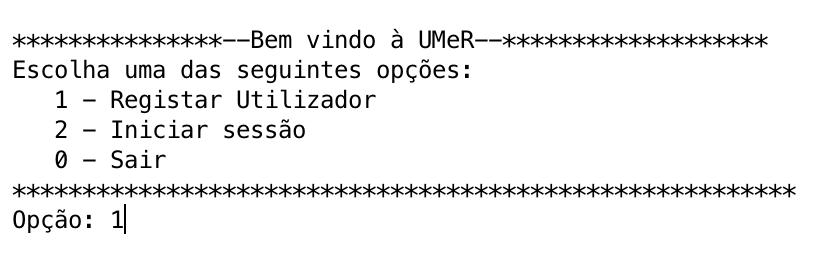
\includegraphics[scale=0.6]{imagem/menuInicial}
\caption{Menu Inicial  }
\label{p3:fig:p2_paginicial}
\end{figure}

\section{Menu Inicial-Registo}

O utilizador consoante o seu tipo poderá efetuar um registo na aplicação. Será apresentado o seguinte menu para o registo de atores no sistema: 

\begin{figure}[htpb]
	\centering
	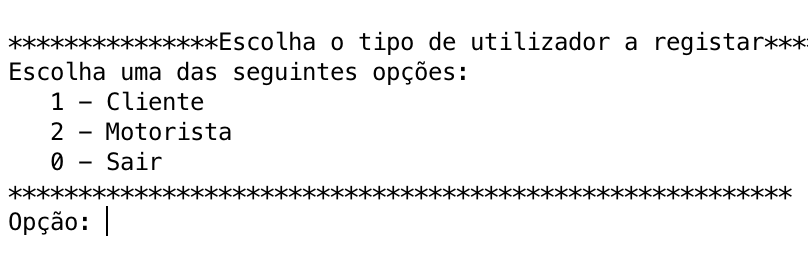
\includegraphics[scale=0.6]{imagem/escolhaTipoAtor}
	\caption{Menu de Registo na Aplicação }
	\label{p3:fig:p2_escolhaTipoAtor}
\end{figure}
Os dados pedidos no ato de registo quer de clientes ou motoristas é o mesmo, no entanto serão guardados de acordo com o tipo inicialmente escolhido. 
\newline

\noindent\begin{minipage}[b]{.4\textwidth}
	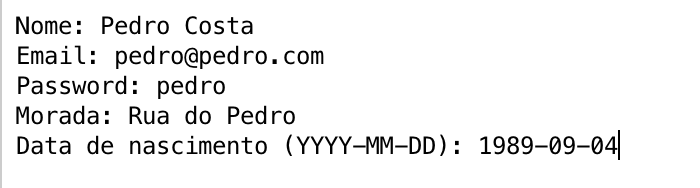
\includegraphics[scale=0.6]{imagem/exemploregistomotorista}
	\small{Exemplo de registo de um motorista}
\end{minipage} 
\hfill
\begin{minipage}[b]{.4\textwidth}
	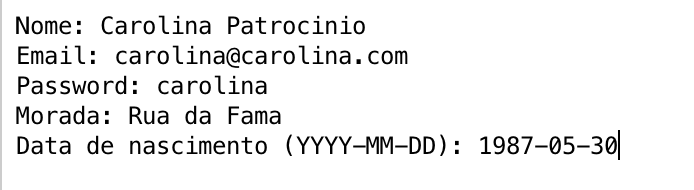
\includegraphics[scale=0.6]{imagem/exemploderegistocliente}
	\small{Exemplo de registo de um cliente}
\end{minipage}
\hfill

\section{Menu Inicial - Iniciar Sessão }
\subsection{Funcionalidades de Cliente}
O Cliente tem à sua disposição várias funcionalidades tais como: Soliciar uma viagem; Visualizar o histórico de viagens; Classificar viagens e ainda Ver e Editar dados pessoais. 
\begin{figure}[htpb]
	\centering
	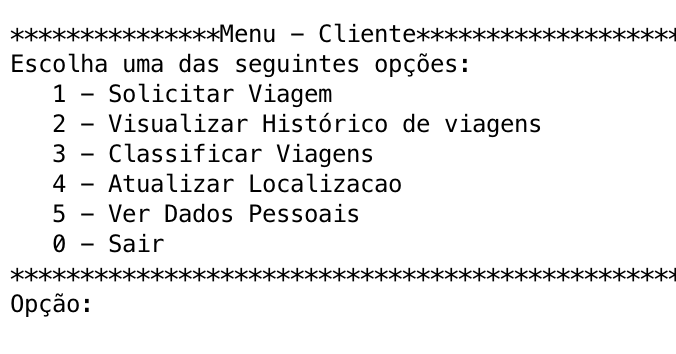
\includegraphics[scale=0.7]{imagem/menuCliente}
	\caption{Menu de Cliente }
	\label{p3:fig:p3_menuCliente}
\end{figure}

\begin{enumerate}
	\item \textbf{Solicitar Viagem}

Ao escolher "Solicitar Viagem" será pedido ao Cliente para introduzir as Coordenadas de destino. Após a inserção das Coordenadas é pedido ao Cliente para escolher se quer o táxi que se encontra mais próximo dele ou se prefere escolher um táxi especifico. 

\noindent\begin{minipage}[b]{.5\textwidth}
	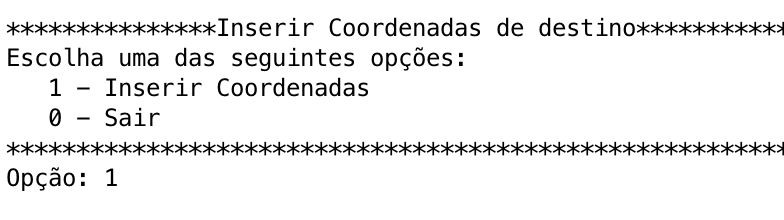
\includegraphics[scale=0.55]{imagem/inserirDestino}
	\small{Menu para inserir as coordenadas}
\end{minipage} 
\hfill
\begin{minipage}[b]{.45\textwidth}
	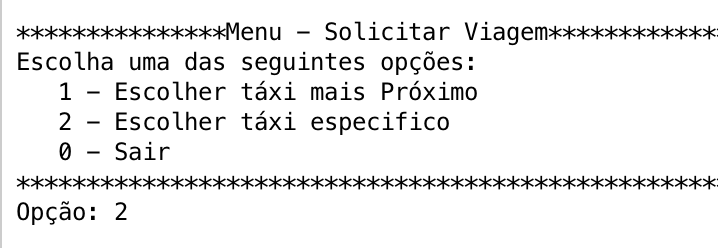
\includegraphics[scale=0.55]{imagem/coorInseridas}
	\small{Menu após a inserção de coordenadas: Escolha de táxi}
\end{minipage}
\hfill

O Cliente após escolher a opção 1, é-lhe apresentado um menu com os dados do táxi que se encontra mais perto da localização do cliente. De seguida é dada a opção de aceitar fazer a viagem ou não. 

\noindent\begin{minipage}[b]{.4\textwidth}
	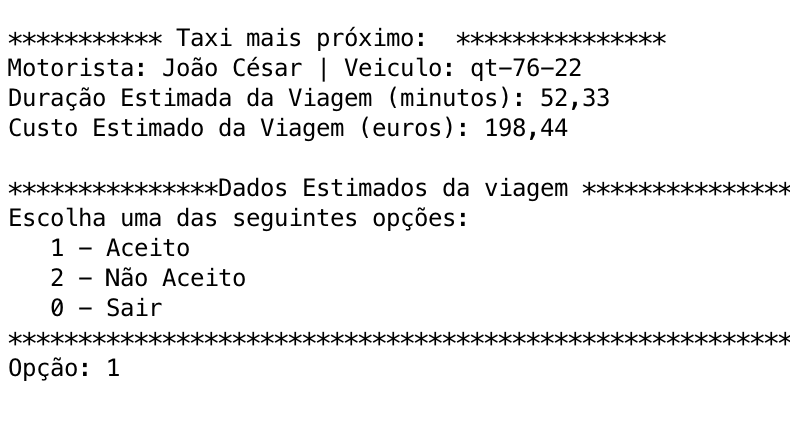
\includegraphics[scale=0.4]{imagem/taxiMaisProx}
	\small{Menu com os dados do taxi mais próximo}
\end{minipage} 
\hfill
\begin{minipage}[b]{.45\textwidth}
	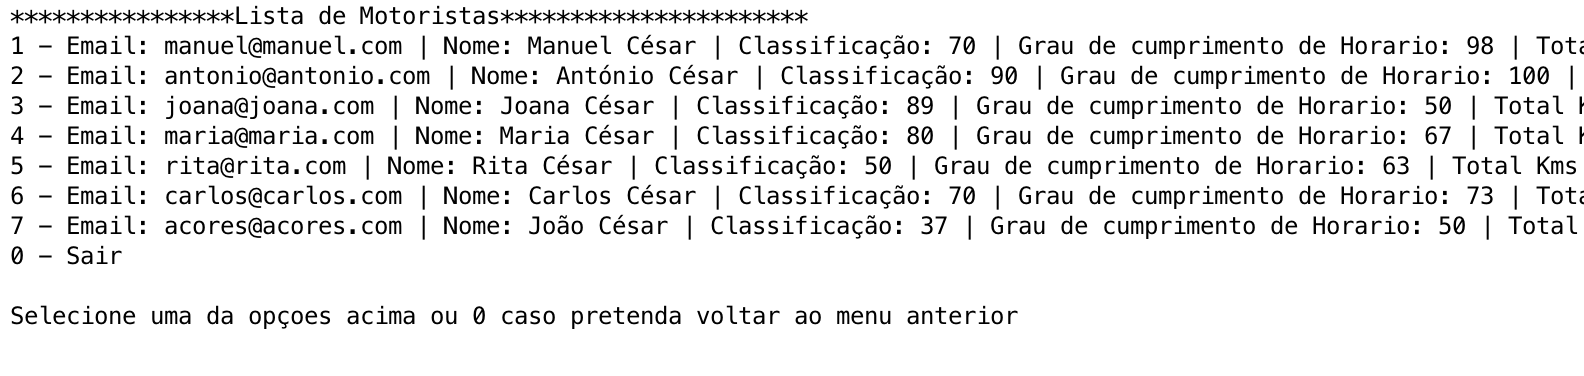
\includegraphics[scale=0.35]{imagem/escolherTaxiEspecifico}
	\small{Menu com os dados dos táxis disponiveis}
\end{minipage}
\hfill

\newpage
Se aceitar fazer a viagem aparecer-lhe-á o seguinte menu, com a informação do tempo que o táxi demorará até chegar à localização do cliente. 

\begin{figure}[htpb]
	\centering
	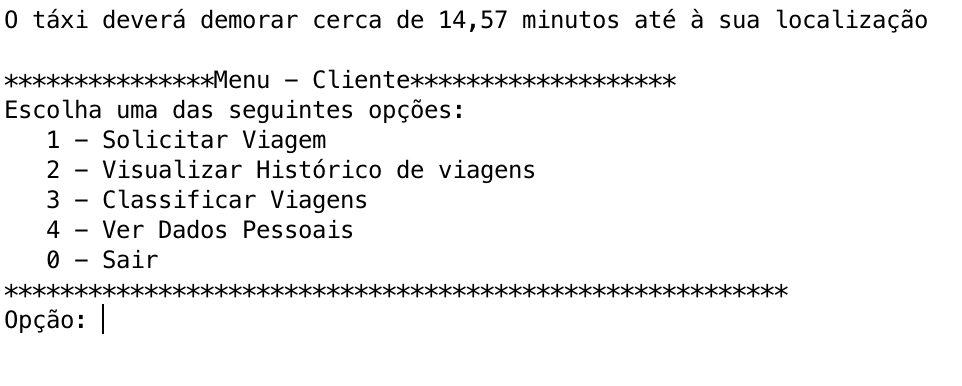
\includegraphics[scale=0.6]{imagem/aceitarViagem}
	\caption{Menu de Viagem aceite }
	\label{p3:fig:p3_aceitarViagem}
\end{figure}

Caso o cliente tenha efetuado uma viagem e esta ainda estiver a decorer, não poderá solicitar outra viagem sem que a atual tenha terminado. Será mostrada uma mensagem como a seguinte: 
\begin{figure}[htpb]
	\centering
	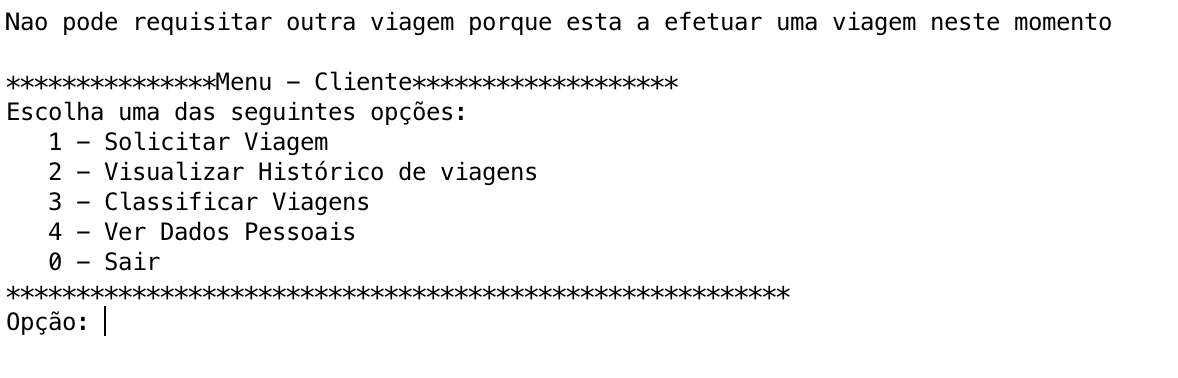
\includegraphics[scale=0.6]{imagem/erroEmViagem}
	\caption{Menu de Erro: Cliente está em viagem }
	\label{p3:fig:p3_erroEmViagem}
\end{figure}


\item \textbf{Visualizar Histórico de viagens }

O Cliente poderá visualizar o seu histórico de todas viagens efetuadas e poderá escolher como quer ver a informação ou entre datas ou todas as viagens. 

\noindent\begin{minipage}[b]{.3\textwidth}
	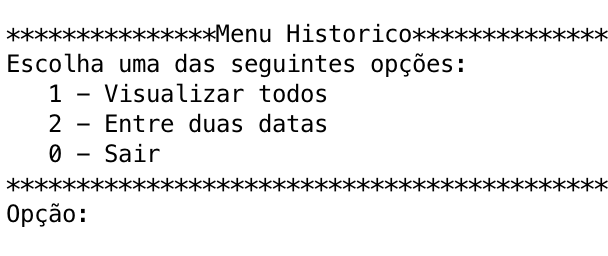
\includegraphics[scale=0.4]{imagem/menuHistorico}
	\small{Menu para escolher como visualizar histórico}
\end{minipage} 
\hfill
\begin{minipage}[b]{.45\textwidth}
	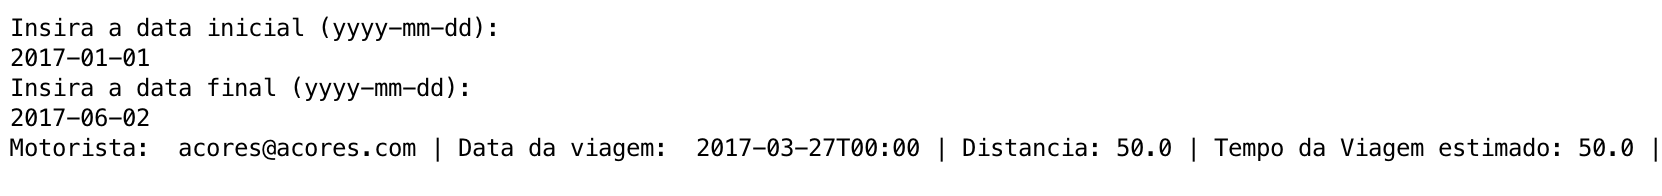
\includegraphics[scale=0.4]{imagem/verHistoricoEntreDatas}
	\small{Menu ver histórico entre datas}
\end{minipage}
\hfill


\newpage
\item \textbf{Classificar Viagens} 

O menu para classificação de viagem, servirá para o cálculo da média de classificação geral do Motorista. 

\noindent\begin{minipage}[b]{.4\textwidth}
	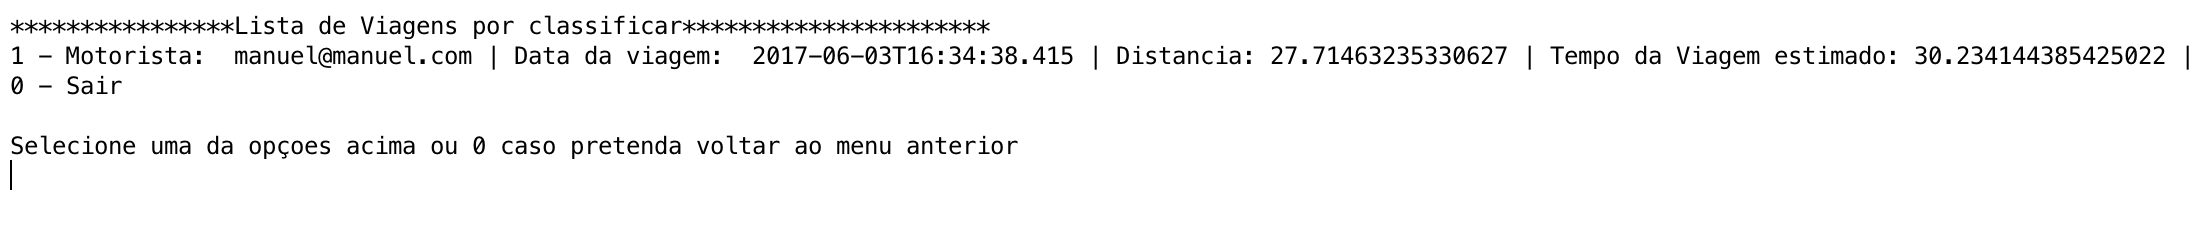
\includegraphics[scale=0.3]{imagem/listaViagensPorClassificar}
	\small{Menu para Cliente classificar a viagem }
\end{minipage} 
\hfill
\begin{minipage}[b]{.4\textwidth}
	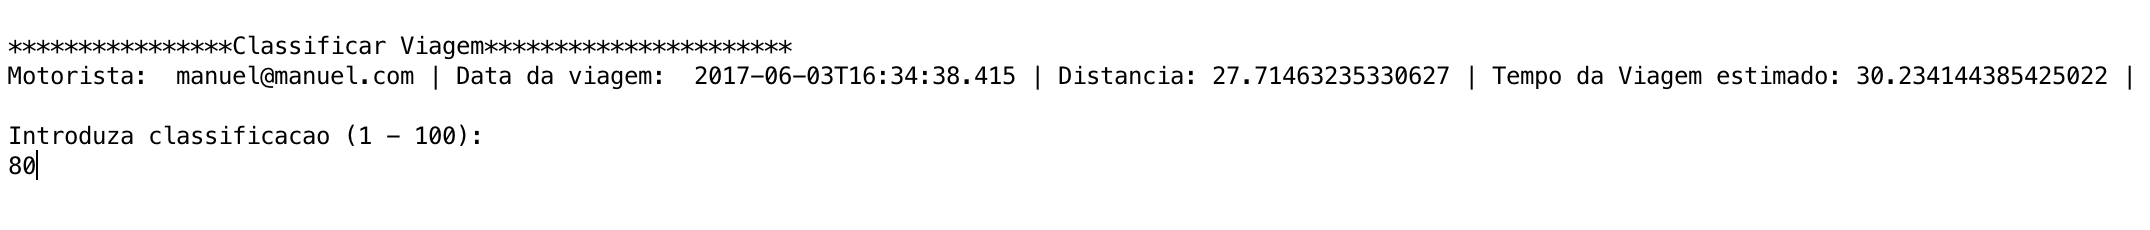
\includegraphics[scale=0.4]{imagem/classificarViagem}
	\small{Menu para classificação da viagem}
\end{minipage}
\hfill


\item \textbf{Atualizar Localização} 

O menu para atualizar localização serve para o cliente após fazer uma viagem, atualizar para uma nova localização em que se encontra para efetuar uma nova viagem. 

\begin{figure}[htpb]
	\centering
	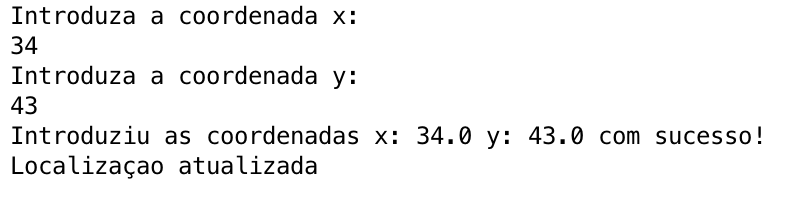
\includegraphics[scale=0.6]{imagem/atualizarLocalizacao}
	\caption{Atualizar Localização}
	\label{p3:fig:p3_atualizarLocalizacao}
\end{figure}



\item \textbf{Ver dados pessoais }

É oferecida aos Clientes e a todos os outros utilizadores a possibilidade de verem os seus dados e editarem todos os campos com a excepção do email. 
\begin{figure}[htpb]
	\centering
	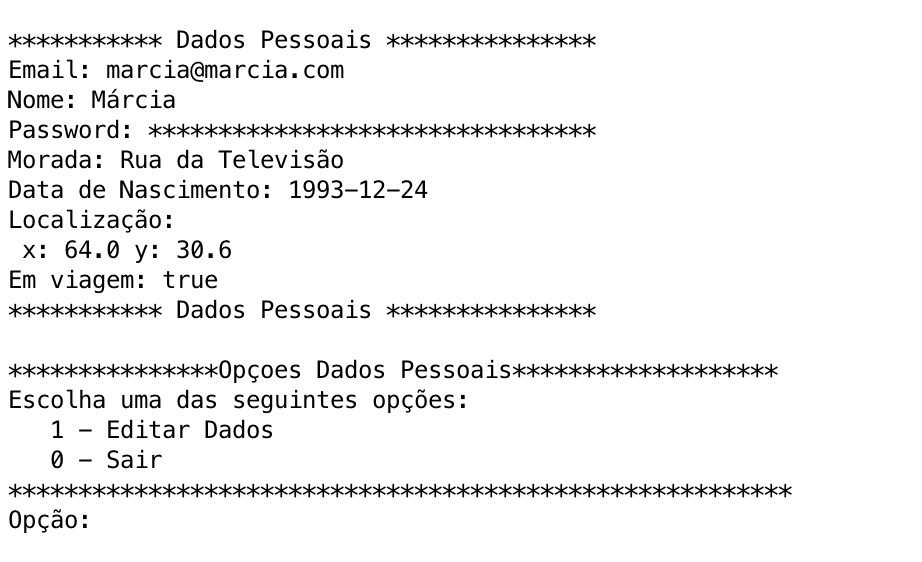
\includegraphics[scale=0.6]{imagem/verDadosPessoais}
	\caption{Menu de visualização e edição dos dados Pessoais }
	\label{p3:fig:p3_verDadosPessoais}
\end{figure}

\end{enumerate}


\newpage
\subsection{Funcionalidades de Motorista}
O motorista na UMeR poderá registar e remover o seu veiculo, gerir viagens é para iniciar uma viagem que esteja pendente; gerir horário de trabalho serve para não aceitar viagens quando não está a trabalhar. Poderá ver o histórico das viagens efetuadas, quais os seus melhores 10 clientes e ver e editar os seus dados pessoais. O menu apresentado será o seguinte: 
\begin{figure}[htpb]
	\centering
	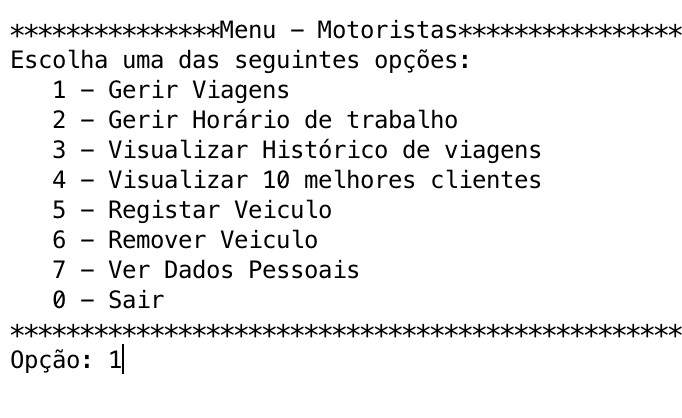
\includegraphics[scale=0.6]{imagem/menuMotorista}
	\caption{Menu de Motorista }
	\label{p3:fig:p3_menuMotorista}
\end{figure}

\begin{enumerate}
	\item \textbf{Gerir Viagens}

Após escolher gerir uma viagem será apresentado o menu com a opção de terminar viagem, caso  Ao efetuar este passo o motorista passa a estar num disponivel, isto é fica apto para receber novas viagens. 

\hfill
\noindent\begin{minipage}[b]{.4\textwidth}
	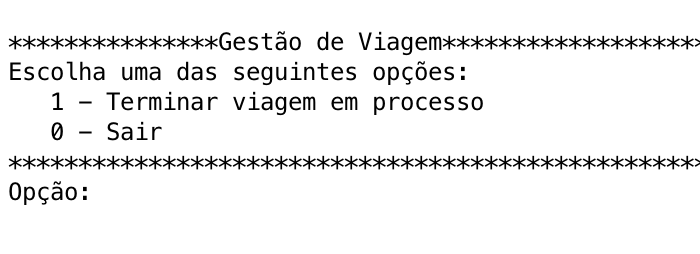
\includegraphics[scale=0.55]{imagem/gerirViagem}
	\small{Menu do motorista para terminar uma viagem}
\end{minipage} 
\hfill
\begin{minipage}[b]{.4\textwidth}
	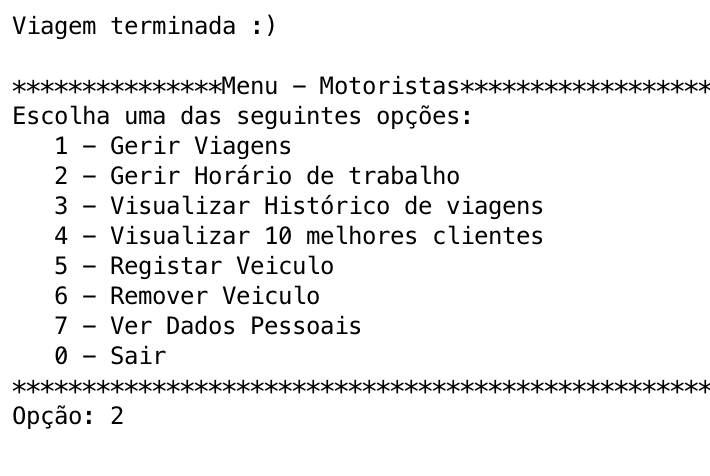
\includegraphics[scale=0.5]{imagem/viagemTerminada}
	\small{Menu após terminar viagem}
\end{minipage}
\hfill 

\item \textbf{Gerir Horário de trabalho}

Na opção de gerir horário de trabalho é apresentado o seguinte menu em que o motorista o poderá terminar. 

\noindent\begin{minipage}[b]{.4\textwidth}
	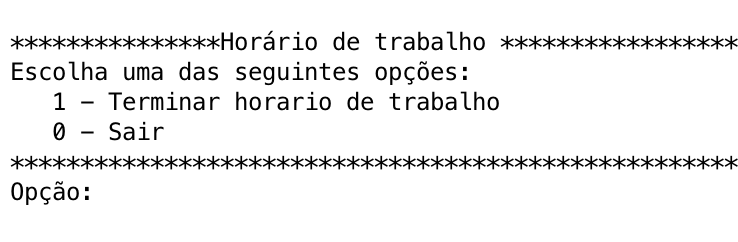
\includegraphics[scale=0.55]{imagem/gerirHorarioTrabalho}
	\small{Menu do motorista para iniciar horario de trabalho}
\end{minipage} 
\hfill
\begin{minipage}[b]{.4\textwidth}
	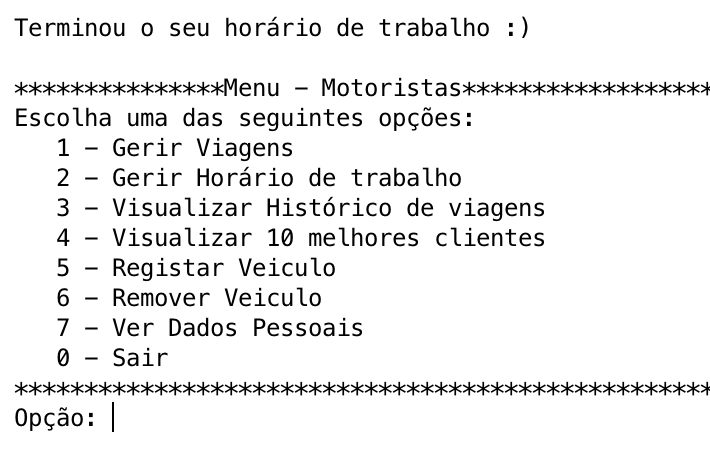
\includegraphics[scale=0.5]{imagem/terminouHorarioTrabalho}
	\small{Menu após terminar horário}
\end{minipage}
\hfill

\newpage

Após terminar o horário, os menus mudam de modo a que o motorista possa voltar ao trabalho, sendo criados para tal os seguintes menus: 

\noindent\begin{minipage}[b]{.4\textwidth}
	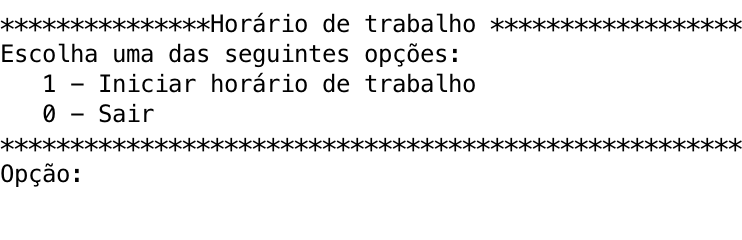
\includegraphics[scale=0.55]{imagem/iniciarHorarioTrabalho}
	\small{Menu do motorista para terminar horario de trabalho}
\end{minipage} 
\hfill
\begin{minipage}[b]{.4\textwidth}
	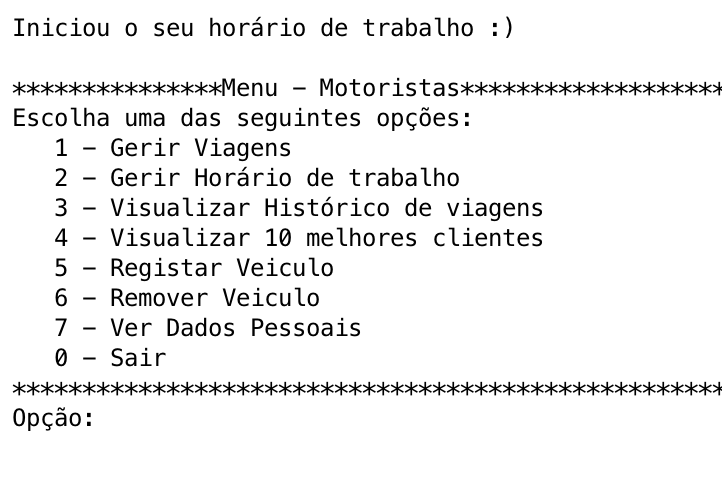
\includegraphics[scale=0.5]{imagem/iniciouHorarioTrabalho}
	\small{Menu após iniciar horário de trabalho}
\end{minipage}
\hfill

\item \textbf{Visualizar Histórico de Viagens}

O menu Visualizar Histórico de viagens permite ao motorista escolher em que tipo de formato prefere ver o histórico ou entre datas ou o total. 
\begin{figure}[htpb]
	\centering
	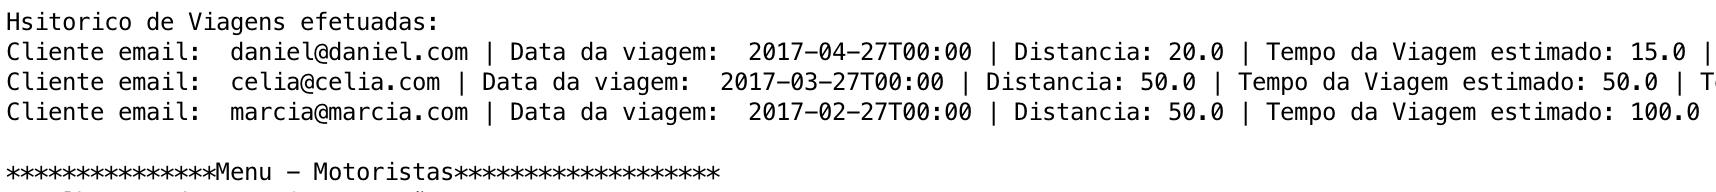
\includegraphics[scale=0.6]{imagem/verViagensMotorista}
	\caption{Menu de visualização de Histórico de viagens}
	\label{p3:fig:p3_verViagensMotorista}
\end{figure}


\item \textbf{Visualizar 10 melhores Clientes}

Esta opção permite ao motorista visualizar quais os seus melhores 10 clientes, isto é os clinetes que gastam mais dinheiro em viagens. 

\begin{figure}[htpb]
	\centering
	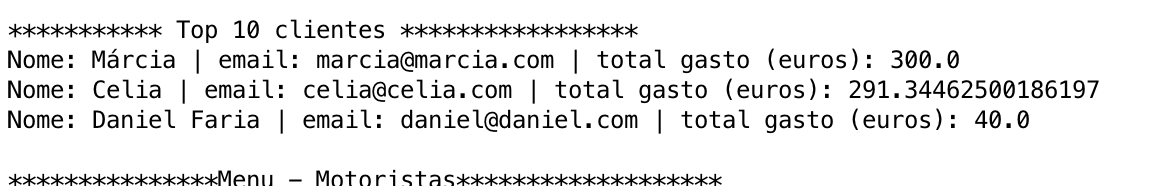
\includegraphics[scale=0.6]{imagem/topClientesMotorista}
	\caption{Menu de visualização de 10 melhores Clientes do Motorista}
	\label{p3:fig:p3_topClientesMotorista}
\end{figure}



\item \textbf{Registar Veiculo}

Esta opção permite ao motorista associar um veiculo a si mesmo. Só é permitido que um um motorista tenha um veiculo associado a si. 

\noindent\begin{minipage}[b]{.4\textwidth}
	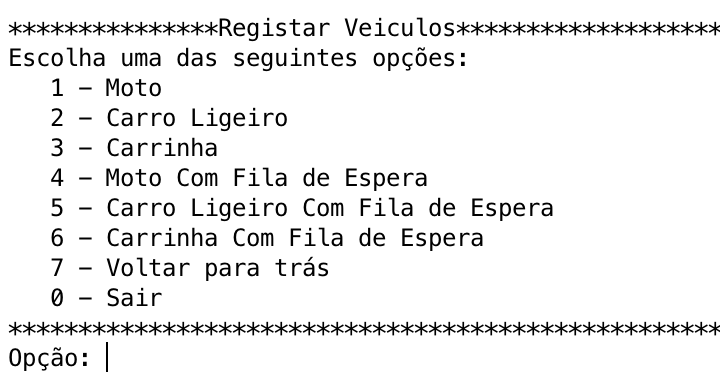
\includegraphics[scale=0.55]{imagem/escolherTipoVeiculo}
	\small{Menu para escolher tipo de veiculo}
\end{minipage} 
\hfill
\begin{minipage}[b]{.4\textwidth}
	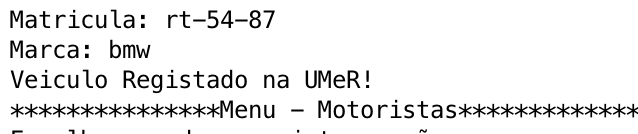
\includegraphics[scale=0.5]{imagem/insercaoDadosVeiculo}
	\small{Menu de inserção de dados no novo veiculo}
\end{minipage}
\hfill


\item \textbf{Remover Veiculo}

Esta opção permite ao motorista remover um veiculo associado a si. 
\begin{figure}[htpb]
	\centering
	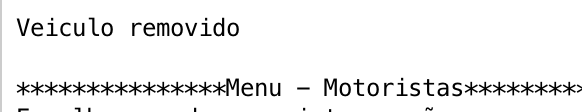
\includegraphics[scale=0.6]{imagem/veiculoRemovido}
	\caption{Menu para remoção do veiculo do motorista}
	\label{p3:fig:p3_veiculoRemovido}
\end{figure}

\end{enumerate}
\subsection{Funcionalidades de Admin}
O Administrador da aplicação tem a funcionalidade principal de visualizar estatísticas, tais como ver uma lista de todos os utilizadores atualizados, os veiculos, o histórico, a lista dos 10 clientes que mais gastam, os motoristas com mais desvios de tempo e custo e ainda poderá ver e editar dados pessoais. 

\begin{figure}[htpb]
	\centering
	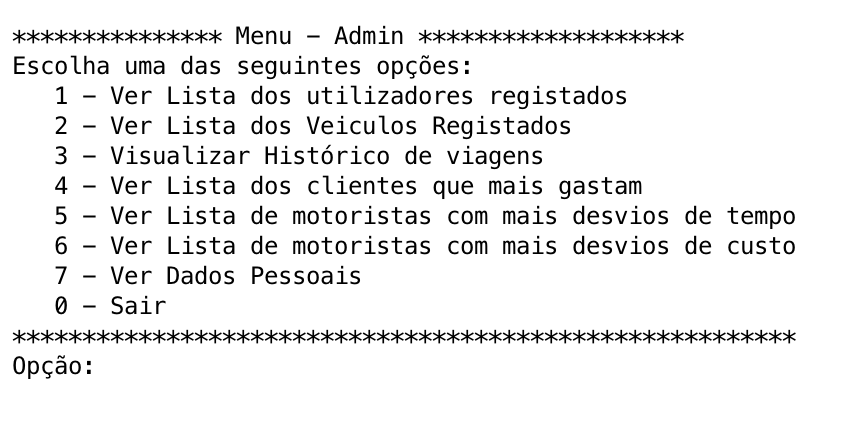
\includegraphics[scale=0.6]{imagem/menuAdmin}
	\caption{Menu do Administrador }
	\label{p3:fig:p3_menuAdmin}
\end{figure}

\newpage
Mostramos de seguida o exemplo de excecução de cada opção do menu: 

\begin{enumerate}
	\item \textbf{Ver lista dos utilizadores Registados}
	\begin{figure}[htpb]
		\centering
		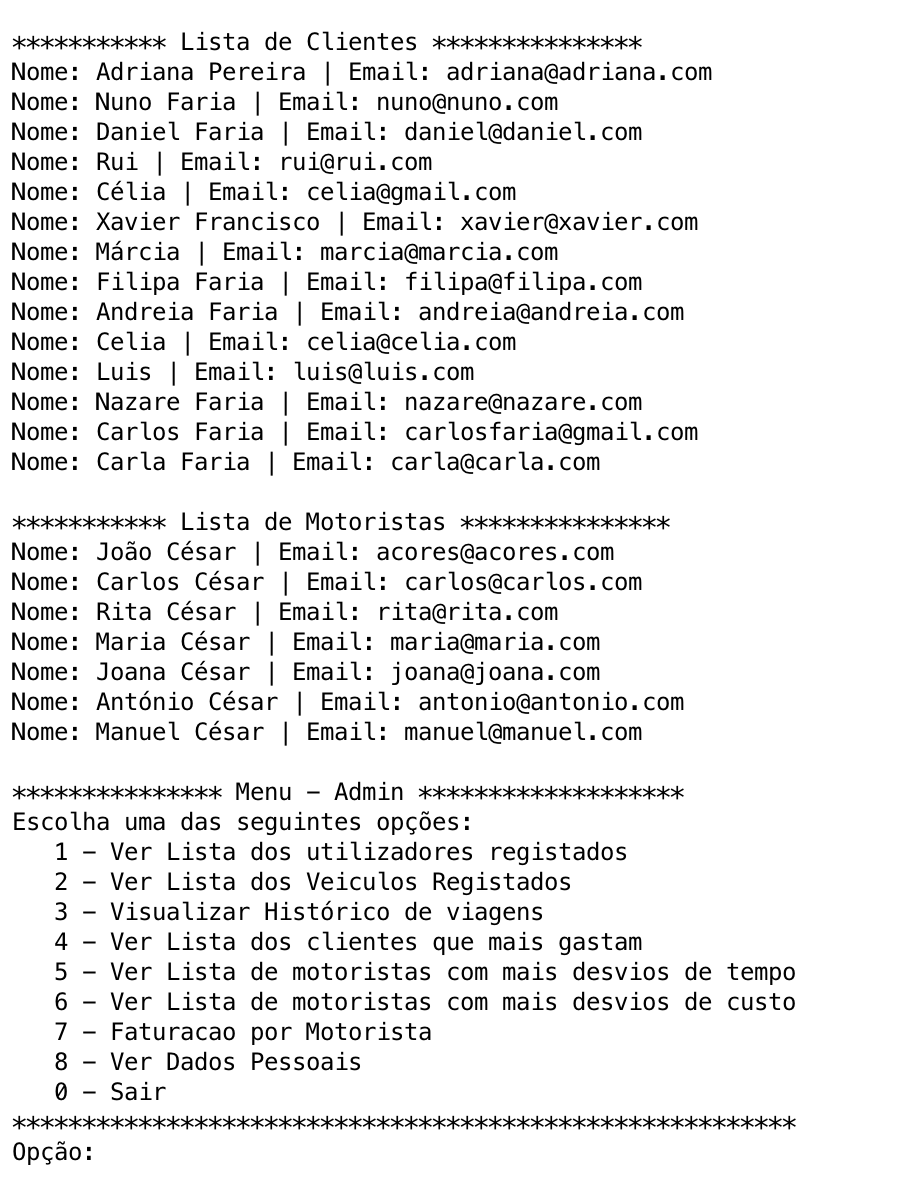
\includegraphics[scale=0.5]{imagem/verListaAtores}
		\caption{Menu do Administrador }
		\label{p3:fig:p3_verListaAtores}
	\end{figure}

\item \textbf{Ver lista dos Veiculos registados }
	\begin{figure}[htpb]
	\centering
	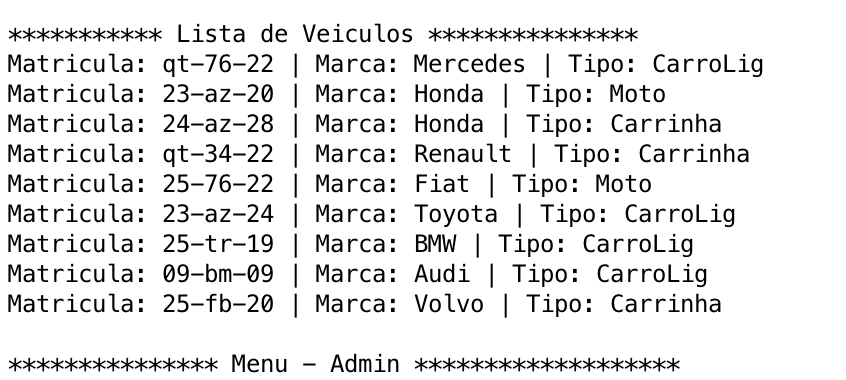
\includegraphics[scale=0.5]{imagem/verListaVeiculos}
	\caption{Ver lista dos veiculos registados }
	\label{p3:fig:p3_verListaVeiculos}
\end{figure}

\newpage
\item \textbf{Visualizar histórico de viagens }

Neste menu o Administrador poderá visualizar todo o histórico ou escolher entre datas, neste caso mostramos como funciona entre datas: 
\begin{figure}[htpb]
	\centering
	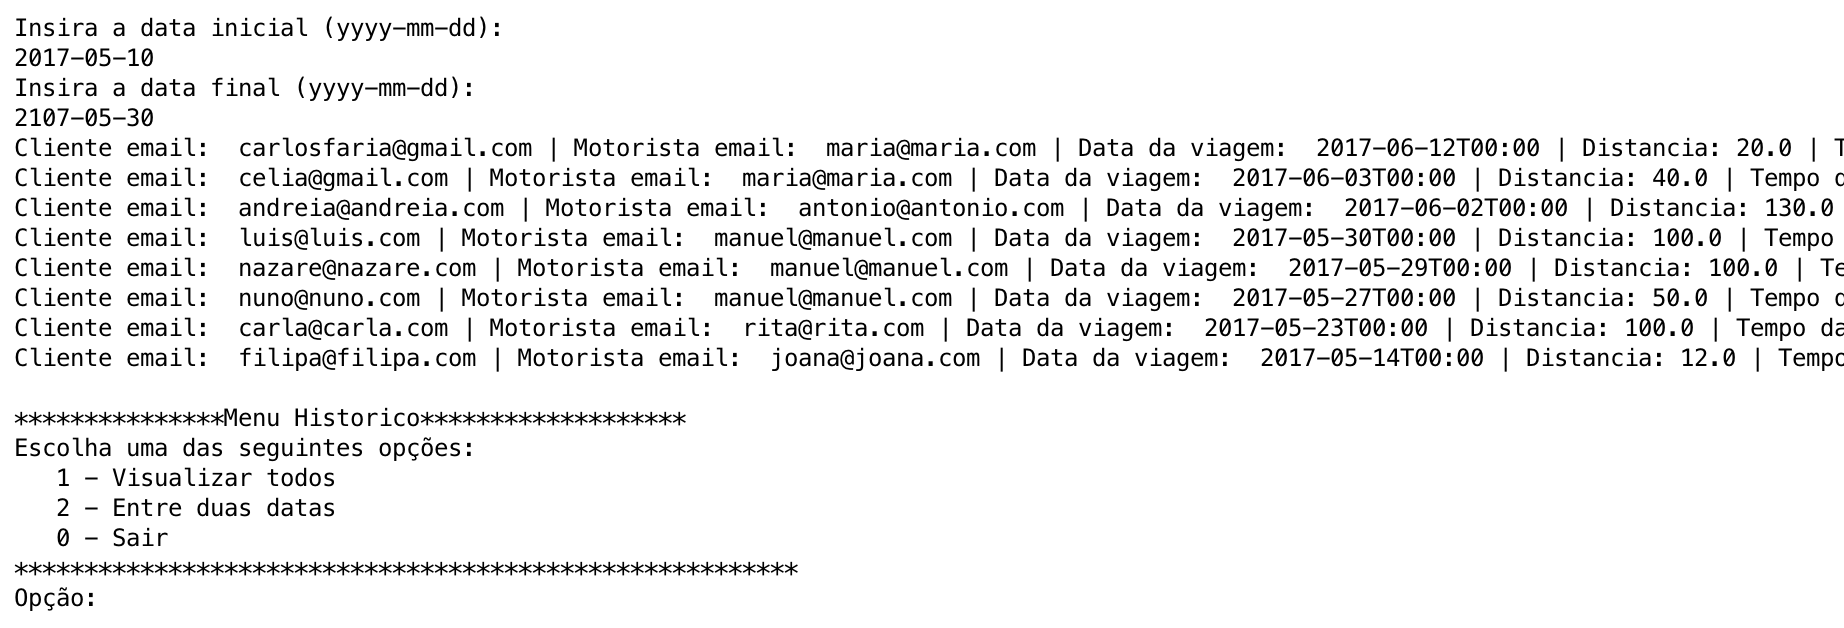
\includegraphics[scale=0.5]{imagem/verListaHistorico}
	\caption{Ver lista de histórico de viagens }
	\label{p3:fig:p3_verListaHistorico}
\end{figure}

\item \textbf{Ver lista dos 10 clientes que mais gastam }

Esta funcionalidade permite listar o top dos 10 melhores clientes da aplicação. 
Este top é construido com base nos históricos terminados (viagens em precurso não são contabilizados para este cálculo). 

\begin{figure}[htpb]
	\centering
	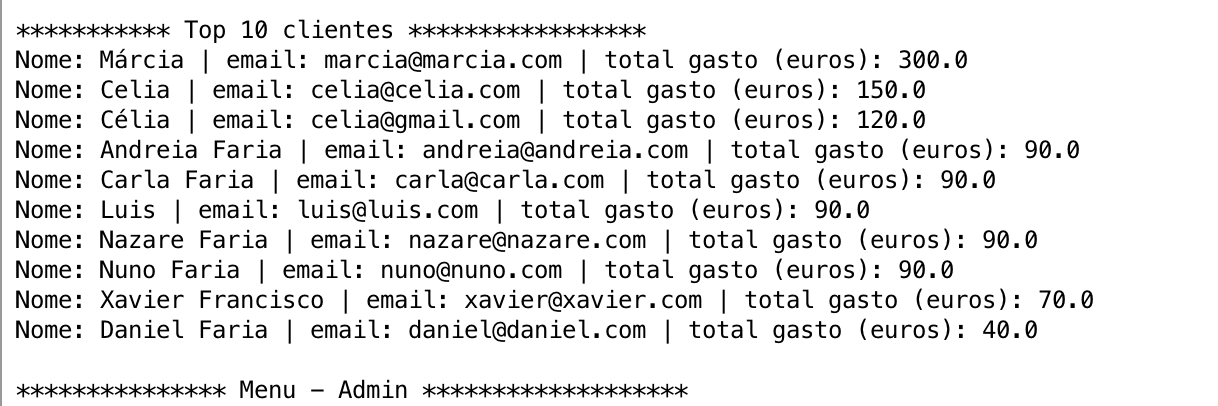
\includegraphics[scale=0.5]{imagem/verClientesMaisGastam}
	\caption{Ver  lista dos 10 clientes que mais gastam  }
	\label{p3:fig:p3_verClientesMaisGastam}
\end{figure}

\item \textbf{Ver lista de motoristas com mais desvios de tempo }

A lista apresentada é ordenada por ordem crescente do grau de cumprimento de tempo. Este valor é calculado com base nos históricos (terminados). Para cada histórico se o tempo estimado for maior que o tempo real, o grau será 100, se o tempo estimado for menor que o tempo real o grau é calculado pela divisão entre o tempo real e o tempo estimado. O grau de cumprimento por motorista é a média do grau de cumprimento dos seus históricos.  

Quanto maior o grau de cumprimento de tempo, melhor será para o cliente uma vez que este grau indica que o motorista efetua viagens com um tempo menor ou igual daquele que foi estimado. 

Para o administradores da plataforma quanto menor o grau de cumprimento de tempo pior uma vez que as viagens demoraram mais tempo do que o estimado e por consequência possibilitará a realização de mesnos viagens (menos faturação). 

\begin{figure}[htpb]
	\centering
	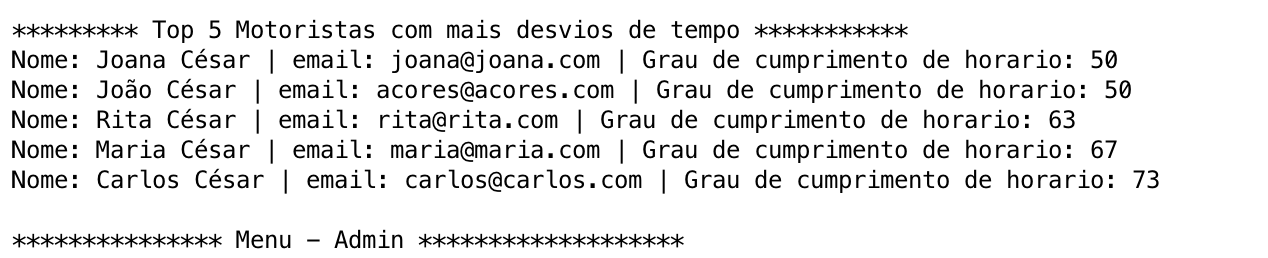
\includegraphics[scale=0.5]{imagem/verMotoristasMaisDesvioTempo}
	\caption{Ver lista de motoristas com mais desvios de tempo }
	\label{p3:fig:p3_verMotoristasMaisDesvioTempo}
\end{figure}

\newpage
\item \textbf{Ver lista de motoristas com mais desvios de custo }

A lista apresentada é ordenada por ordem crescente do grau de cumprimento de custo. Este valor é calculado com base nos históricos (terminados). Para cada histórico se o custo real for maior que o custo estimado, o grau será 100, se o custo real for menor que o custo estimado o grau é calculado pela divisão entre o custo real  e o custo estimado. O grau de cumprimento por motorista é a média do grau de cumprimento dos seus históricos.  

Quanto menor o grau de cumprimento de custo, melhor será para o cliente uma vez que este grau indica que o motorista efetua viagens com um custo menor do que aquele que foi estimado. 

Para o administradores da plataforma quanto menor o grau de cumprimento de custo pior uma vez que as receitas serão menores em relação às receitas estimadas. 


\begin{figure}[htpb]
	\centering
	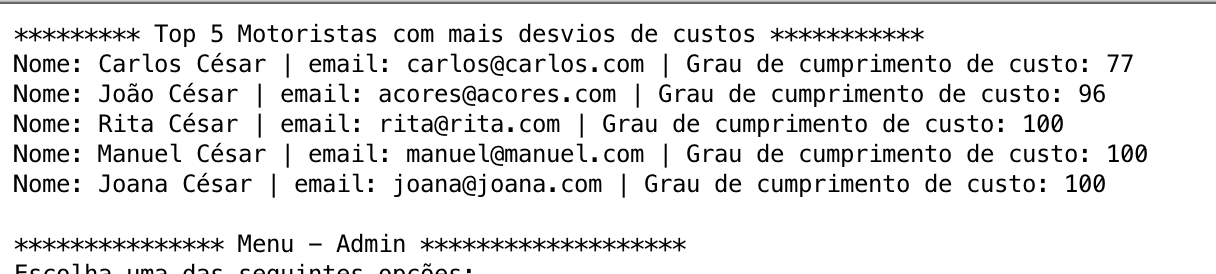
\includegraphics[scale=0.5]{imagem/verMotoristasMaisDesvioCusto}
	\caption{Ver lista de motoristas com mais desvios de custos}
	\label{p3:fig:p3_verMotoristasMaisDesvioCusto}
\end{figure}

\item\textbf{ Faturação por Motorista}

Esta funcionalidade permite ver os dados entre datas ou a lista com todos os dados. Decidiu-se que faria mais sentido apresentar a faturação por motorista, visto que o motorista só tem um veiculo então a informação seria a mesma. 

\begin{figure}[htpb]
	\centering
	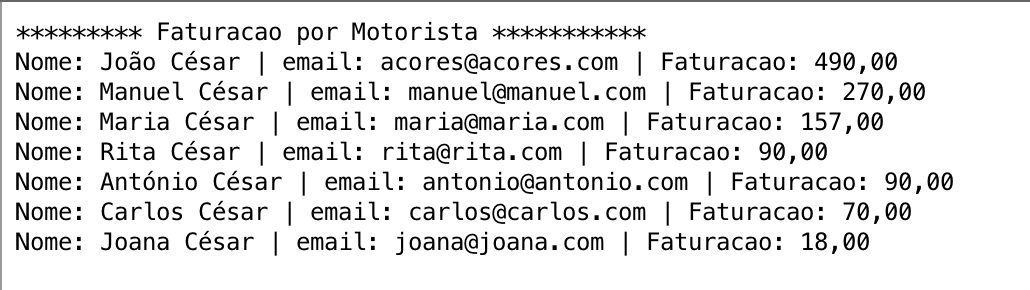
\includegraphics[scale=0.5]{imagem/faturacaoPorMotorista}
	\caption{Ver faturação por motorista}
	\label{p3:fig:p3_faturacaoPorMotorista}
\end{figure}

	
\end{enumerate}

